\documentclass[11pt,a4paper]{article}

\usepackage[margin=0.95in]{geometry}
\usepackage[T1]{fontenc}
\usepackage{lmodern}
\usepackage{amsmath,amssymb,amsthm,mathtools}
\usepackage{booktabs,array}
\usepackage{graphicx}
\usepackage{xcolor}
\usepackage{xurl}
\usepackage[colorlinks=true,linkcolor=blue!65!black,citecolor=teal!70!black,urlcolor=blue!65!black]{hyperref}
\usepackage{microtype}

\newtheorem{theorem}{Theorem}
\newtheorem{proposition}[theorem]{Proposition}
\newtheorem{lemma}[theorem]{Lemma}
\newtheorem{corollary}[theorem]{Corollary}
\theoremstyle{remark}
\newtheorem{remark}[theorem]{Remark}

\newcommand{\supp}{\operatorname{supp}}
\newcommand{\lcm}{\operatorname{lcm}}
\newcommand{\den}{\operatorname{den}}
\newcommand{\TV}{\operatorname{TV}}
\newcommand{\DKL}{D_{\mathrm{KL}}}
\newcommand{\Unif}{\mathrm{Unif}}
\newcommand{\Q}{\mathbb{Q}}
\newcommand{\Z}{\mathbb{Z}}
\newcommand{\R}{\mathbb{R}}

\title{\textbf{Exponential Bit-Complexity Tightening, Optimal \texorpdfstring{$b$}{b}-ary\\
Matching Trees, and Exact Sharp Support Thresholds for\\
Normal-Form Correlated Equilibria in Extensive-Form Games}}

\author{Lluis Eriksson\thanks{Independent researcher. Authored by Lluis Eriksson with AI-assisted formal verification, exact-arithmetic software generation, and mathematical drafting (Google Antigravity). Manuscript and figures licensed CC-BY-4.0; verification repository, Lean~4 formalization, and exact rational certificates licensed MIT at \nolinkurl{https://github.com/lluiseriksson/extensive-form-nfce-sharp-gap-and-hardness}.}}
\date{November 26, 2026}

\begin{document}
\maketitle

\begin{abstract}
In a recent breakthrough, Cheval, Horn, Paul, and Shirmohammadi (\nolinkurl{arXiv:2611.34897v1}) proved that computing an exact Normal-Form Correlated Equilibrium (NFCE) of quadratic support size in a perfect-recall extensive-form game belongs to PPAD, and that the prescribed-support exact search problems for two players under dimension-based ($\kappa_d = (d_1+1)(d_2+1)$) and node-based ($\kappa_V = \lfloor |V|^2/36 \rfloor$) support caps are PPAD-complete. We establish three sharp structural, complexity-theoretic, and combinatorial advances over this framework.
First (Theorem~\ref{thm:lp_gap}), by eliminating zero-weight columns at optimal LP vertices, leaving the probability-simplex row unscaled, and replacing the raw payoff/chance denominator product $B = \prod_{r\in R}\den(r)$ with per-player leaf-payoff least common multiples $D_i = \lcm_{z\in Z}\den(p_c(z)u_i(z))$, we tighten the uniform rational LP reweighting gap of Lemma~14 from $((K+1)B)^{-(K+1)}$ to $(\sqrt{K}(K+1)^{K/2}D_{\max}^K)^{-1}$. This saves more than $\frac{K}{2}\log_2(K+1) + K\log_2(B/D_{\max})$ bits of weak-Nash oracle precision ($>30\times$ fewer bits on the authors' matching-tree instances at $r=8, q=10$), while certifying exact two-player support dominance $K - \kappa_d = d_1^2 + d_2^2 - d_1 d_2 \ge \frac{1}{2}(d_1^2 + d_2^2)$ ($2\times$ balanced reduction).
Second (Theorem~\ref{thm:bary}), generalizing the binary matching branch to arbitrary $b$-ary perfect-recall trees $M_b(k)$ ($m = b^k$) shows that sequence-form dimensions $d_1 = d_2 = m + r - 2$ are invariant of $b$ while node overhead $f(b) = b + 2 + \frac{2}{b-1} = 6 + \frac{(b-2)(b-3)}{b-1}$ achieves its unique integer minimum $f(b) = 6$ if and only if $b \in \{2, 3\}$. This proves that Corollary~20's $1/36$ node-quadratic constant is exact and unimprovable across all $b$-ary matching trees, and that ternary trees ($b=3$) achieve the identical minimal node count $6m + r^2 + r - 3$ while exponentially reducing the pure-strategy space from $r\,2^{m-1}$ to $r\,3^{(m-1)/2}$ ($>10^{15}\times$ smaller at $m=243$).
Third (Theorem~\ref{thm:hardness}), we shrink the PPAD-hardness matching trees by $\ge 8\times$ in the dimension-based reduction ($m > r^2(r-1)$ vs.\ $8r^3$) and $32\times$--$64\times$ in the node-based reduction ($m > r^2(r^2+r-3)/6$ vs.\ $8r^4$), incorporate the Kullback--Csisz\'ar--Kemperman refined Pinsker bound, and prove an exact minimum-support dichotomy: an exact NFCE of support $m^2$ exists on $\Gamma_b(P,Q,k)$ if and only if $(P,Q)$ admits an exact Nash equilibrium with probabilities in $\frac{1}{m}\Z$, separating ternary from binary trees on an explicit asymmetric $2{\times}2$ game $G_{1/3}$. All algebraic and combinatorial cores are formalized constructively in zero-dependency Lean~4.35.0 ($18$ theorems, $0$ \texttt{sorry}, $0$ \texttt{Classical.choice}) and verified by an AST-audited zero-float Python verifier issuing $16$ SHA-256 certificates.
\end{abstract}

\section{Introduction}\label{sec:intro}

Normal-Form Correlated Equilibrium (NFCE) in extensive-form games~\cite{vonStengelForges2008} requires obedience with respect to full normal-form strategy plans chosen prior to play, making its equilibrium polytope exponentially large in the game tree. In~\cite{CHPS2026}, Cheval, Horn, Paul, and Shirmohammadi resolved a major open problem by placing exact NFCE computation in PPAD~\cite{Papadimitriou1994,CDT2009} via a three-stage pipeline: (i)~compute a weak $\epsilon_\Gamma$-Nash equilibrium via a PPAD oracle; (ii)~compress its realization-equivalent product into a support $S$ of size at most $K = 1 + \sum_{i=1}^n d_i(d_i+1)$ using Carath\'eodory's theorem on the feature-expectation polytope; and (iii)~solve a compact sequence-form reweighting LP~\cite{KollerMegiddo1992,KMS1996} at $t=0$, guaranteed feasible whenever $\epsilon_\Gamma < \eta$ where $\eta = ((K+1)B)^{-(K+1)}$ is a uniform rational vertex gap (Lemma~14 / Theorem~6). For two players, they further establish PPAD-completeness under quadratic support caps $\kappa_d = (d_1+1)(d_2+1)$ and $\kappa_V = \lfloor |V|^2/36 \rfloor$ using a public-coin reduction combining an $r{\times}r$ bimatrix game $(P,Q)$ with a binary matching tree $M$ ($m = 2^k$).

This work establishes sharp quantitative and structural improvements across every stage of~\cite{CHPS2026} (summarized in Table~\ref{tab:summary}):
\begin{enumerate}
  \item \textbf{Active-support LCM--Hadamard LP-gap tightening (Section~\ref{sec:lp_gap}):} Replacing $B$ by per-player LCMs $D_i$ and exploiting active-support sparsity eliminates a full factor $(K+1)B$, takes the square root of the $(K+1)^K$ factor, and yields an unboundedly growing multiplicative bit-precision reduction on the matching-tree family itself.
  \item \textbf{Optimal $b$-ary matching trees and sharpness of $1/36$ (Section~\ref{sec:bary}):} Analyzing general $b$-ary matching trees $M_b(k)$ proves that $b \in \{2,3\}$ are the unique integer minimizers of node overhead $f(b) = 6$, certifying that $1/36$ cannot be improved by changing branching arity while revealing that ternary trees ($b=3$) exponentially compress the pure-strategy space.
  \item \textbf{$8\times$--$64\times$ hardness tree tightening and exact $m^2$-support dichotomy (Section~\ref{sec:hardness}):} Tightening the Pinsker threshold shrinks the dimension-based and node-based hardness trees by $\ge 8\times$ and $32\times$--$64\times$, and a rectangle-rigidity proof characterizes exactly when the minimal support floor $m^2$ is attained.
\end{enumerate}

\begin{table}[htbp]
\centering
\caption{Quantitative and structural advances over Cheval--Horn--Paul--Shirmohammadi~\cite{CHPS2026}.}
\label{tab:summary}
\scriptsize
\setlength{\tabcolsep}{4pt}
\begin{tabular}{@{} >{\raggedright\arraybackslash}p{0.25\textwidth} >{\raggedright\arraybackslash}p{0.32\textwidth} >{\raggedright\arraybackslash}p{0.38\textwidth} @{}}
\toprule
\textbf{Stage / Quantity} & \textbf{CHPS (\nolinkurl{arXiv:2611.34897v1})} & \textbf{This Work (Theorems~\ref{thm:lp_gap}--\ref{thm:hardness})} \\
\midrule
Rational LP gap $\eta$ (Lem.~14) & $((K+1)B)^{-(K+1)}$ & $(\sqrt{K}(K+1)^{K/2}D_{\max}^K)^{-1}$ ($>30\times$ fewer bits at $r=8,q=10$) \\
2-player support cap & $K = 1+d_1(d_1+1)+d_2(d_2+1)$ & Exact gap $K-\kappa_d = d_1^2+d_2^2-d_1d_2 \ge \frac{1}{2}(d_1^2+d_2^2)$ ($2\times$ at $d_1=d_2$) \\
Matching tree arity $b$ & Binary ($b=2$) only & Unique optima $b\in\{2,3\}$ ($f(b)=6$, sharp $1/36$); $b=3$ cuts $|\Sigma_i|$ by $(4/3)^{(m-1)/2}$ \\
Dim-based hardness $m$ & $2^{\lceil\log_2(8r^3)\rceil}$ & $2^{\lceil\log_2(r^2(r-1)+1)\rceil}$ ($\ge 8\times$ smaller $\forall r\ge 2$) \\
Node-based hardness $m$ & $2^{\lceil\log_2(8r^4)\rceil}$ ($r\ge 5$) & $2^{\lceil\log_2(\lfloor r^2(r^2+r-3)/6\rfloor + 1)\rceil}$ ($32\times$--$64\times$ smaller) \\
Minimal support $|\supp|=m^2$ & Lower bound $|\supp|\ge m^2$ only & Exact iff: $(P,Q)$ has a $\frac{1}{m}\Z$-rational Nash; $b=3$ vs $b=2$ split on $G_{1/3}$ \\
\bottomrule
\end{tabular}
\end{table}

\section{Exponential LP-Gap Bit-Complexity Tightening and Support Dominance}\label{sec:lp_gap}

Let $\Gamma$ be an $n$-player perfect-recall extensive-form game with normalized terminal payoffs $u_i(z) \in [0,1]$, sequence-form dimensions $d_i$, and quadratic support bound $K = 1 + \sum_{i=1}^n d_i(d_i+1)$. For each player $i \in [n]$, define the \emph{per-player leaf-payoff least common multiple}
\begin{equation}\label{eq:Di_def}
  D_i := \lcm_{z \in Z} \den\bigl(p_c(z) u_i(z)\bigr), \qquad D_{\max} := \max_{i \in [n]} D_i.
\end{equation}
For any nonempty support $S \subseteq \Sigma$ with $|S| \le K$, the reweighting LP~(11) of~\cite{CHPS2026} minimizes $t \in [0,1]$ over $\mu \in \Delta(S)$ subject to $R_{i,\sigma_i,\sigma'_i}(\mu) \le t$ for all $i$, $\sigma_i \in A_i$, and $\sigma'_i \in \Sigma_i$.

\begin{theorem}[Active-support LCM--Hadamard LP gap and two-player support dominance]\label{thm:lp_gap}
Let $\Gamma$ be any normalized $n$-player perfect-recall extensive-form game and let $S \subseteq \Sigma$ be any nonempty support with $|S| \le K$.
\begin{enumerate}
  \item[\textup{(a)}] \textbf{Sharp active-support LCM--Hadamard vertex gap:} At any optimal vertex $x^* = (\mu^*, t^*)$ of LP~(11) with $t^*(S) > 0$ and active support size $s := |\supp(\mu^*)| \le |S| \le K$,
  \begin{equation}\label{eq:eta_sharp}
    t^*(S) \;\ge\; \eta_{\mathrm{sharp}}(s) := \frac{1}{\sqrt{s}\,(s+1)^{s/2}\prod_{j=1}^{s} D_{i_j}}
    \;\ge\; \eta_{\mathrm{sharp}} := \frac{1}{\sqrt{K}\,(K+1)^{K/2}\,D_{\max}^{K}}.
  \end{equation}
  Consequently, setting $\epsilon_\Gamma^{\mathrm{sharp}} := \frac{1}{2}\eta_{\mathrm{sharp}}$ suffices for exact reweighting in Theorem~6 of~\cite{CHPS2026}: every unnormalized $\epsilon_\Gamma^{\mathrm{sharp}}$-NFCE supported on $S$ can be reweighted in polynomial bit time to an exact rational NFCE supported on $S$.
  \item[\textup{(b)}] \textbf{Strict bit-precision reduction:} For every $1 \le s \le K$ and $1 \le D_{\max} \le B := \prod_{r\in R}\den(r)$, $\eta_{\mathrm{sharp}}(s) > \eta_{\mathrm{CHPS}} = ((K+1)B)^{-(K+1)}$ strictly, saving at least
  \begin{equation}\label{eq:bit_saving}
    \log_2\!\left(\frac{\eta_{\mathrm{sharp}}}{\eta_{\mathrm{CHPS}}}\right)
    \;\ge\; \frac{K+1}{2}\log_2(K+1) + \log_2 B + K\log_2\!\left(\frac{B}{D_{\max}}\right)
  \end{equation}
  bits of oracle precision. In particular, on CHPS's matching-tree game $\Gamma_2(P,Q,k)$ with $r{\times}r$ rational payoffs of common denominator $q$, $D_{\max} \le 2q$ is independent of $m$, whereas $B \ge 2\,q^{2r^2}$, reducing required oracle precision at support cap $\kappa_d$ ($m = m_d^*(r,2)$) by $>30\times$ at $r=8, q=10$ (certified lower bound $30.62\times$ in \texttt{C02}, continuous ratio $33.3\times$ in Figure~\ref{fig:lpgap}(a)).
  \item[\textup{(c)}] \textbf{Exact two-player support dominance:} For every two-player game with dimensions $(d_1,d_2) \neq (0,0)$, the product support $\kappa_d = (d_1+1)(d_2+1)$ strictly beats $K$ with exact gap
  \begin{equation}\label{eq:two_p_gap}
    K - \kappa_d = d_1^2 + d_2^2 - d_1 d_2 = \frac{1}{2}(d_1 - d_2)^2 + \frac{1}{2}(d_1^2 + d_2^2) \ge \frac{1}{2}(d_1^2 + d_2^2) > 0,
  \end{equation}
  achieving a $2\times$ support reduction along $d_1 = d_2$ (Figure~\ref{fig:lpgap}(b)), and replacing $K$ by $\kappa_d$ in~\eqref{eq:eta_sharp} halves the LP-gap exponent as well.
\end{enumerate}
\end{theorem}

\begin{proof}
For (a), let $x^* = (\mu^*, t^*)$ be an optimal vertex with $t^* > 0$ and $s = |\supp(\mu^*)| \ge 1$. Since $t^* > 0$, the constraint $t = 0$ is inactive; if $t^* = 1$ then~\eqref{eq:eta_sharp} holds trivially since $\eta_{\mathrm{sharp}}(s) \le 1$. Thus we may assume $0 < t^* < 1$, so the $|S| + 1$ linearly independent active constraints at $x^*$ consist of: (i)~$|S| - s$ coordinate-zero equations $\mu(\tau) = 0$ for $\tau \notin \supp(\mu^*)$; (ii)~the probability-simplex equation $\sum_{\tau\in S}\mu(\tau) = 1$; and (iii)~$s$ active regret equalities $\sum_{\tau\in S} R_{j}(\tau)\mu(\tau) - t = 0$ ($j = 1,\dots,s$), where row $j$ belongs to some player $i_j \in [n]$.

Eliminating the $|S| - s$ zero variables $\mu(\tau) = 0$ leaves a nonsingular $(s+1){\times}(s+1)$ linear system $M_s y = e_1$ (where $y = (\mu^*|_{\supp(\mu^*)}, t^*)^T$ and $e_1 = (1,0,\dots,0)^T$). Its first row is $(1,\dots,1,0)$, which is already integral with Euclidean norm $\sqrt{s}$. For each regret row $j \in \{1,\dots,s\}$, every pure-profile deviation difference $R_j(\tau) = \sum_{z\in Z} p_c(z) u_{i_j}(z)(\chi_{i_j}(\sigma'_j,z) - \chi_{i_j}(\sigma_j,z))\prod_{r\neq i_j}\chi_r(\tau_r,z)$ satisfies $|R_j(\tau)| \le 1$ and $D_{i_j} R_j(\tau) \in \Z$. Multiplying row $j$ by $D_{i_j}$ (and leaving row~$0$ unscaled) yields an equivalent nonsingular integer system $A_s y = e_1$ whose $j$-th regret row has Euclidean norm at most $D_{i_j}\sqrt{s+1}$. By Cramer's rule, $t^* = \det(A_{s,t})/\det(A_s)$ with $|\det(A_{s,t})| \ge 1$ (since $A_{s,t}$ is integral and $t^* > 0$). Applying Hadamard's inequality to the rows of $A_s$ yields
\[
  |\det(A_s)| \;\le\; \sqrt{s}\prod_{j=1}^{s}\bigl(D_{i_j}\sqrt{s+1}\bigr) = \sqrt{s}\,(s+1)^{s/2}\prod_{j=1}^{s} D_{i_j},
\]
proving~\eqref{eq:eta_sharp}. Strict dominance over $\eta_{\mathrm{CHPS}}$ and~\eqref{eq:bit_saving} follow directly by taking logarithms (squared-integer dominance formalized in Lean~4 as \nolinkurl{sharp_lp_gap_strictly_dominates_chps}), and~\eqref{eq:two_p_gap} is verified in Lean~4 as \nolinkurl{two_player_support_gap_exact} and \nolinkurl{two_player_balanced_support_factor}.
\end{proof}

\begin{figure}[htbp]
\centering
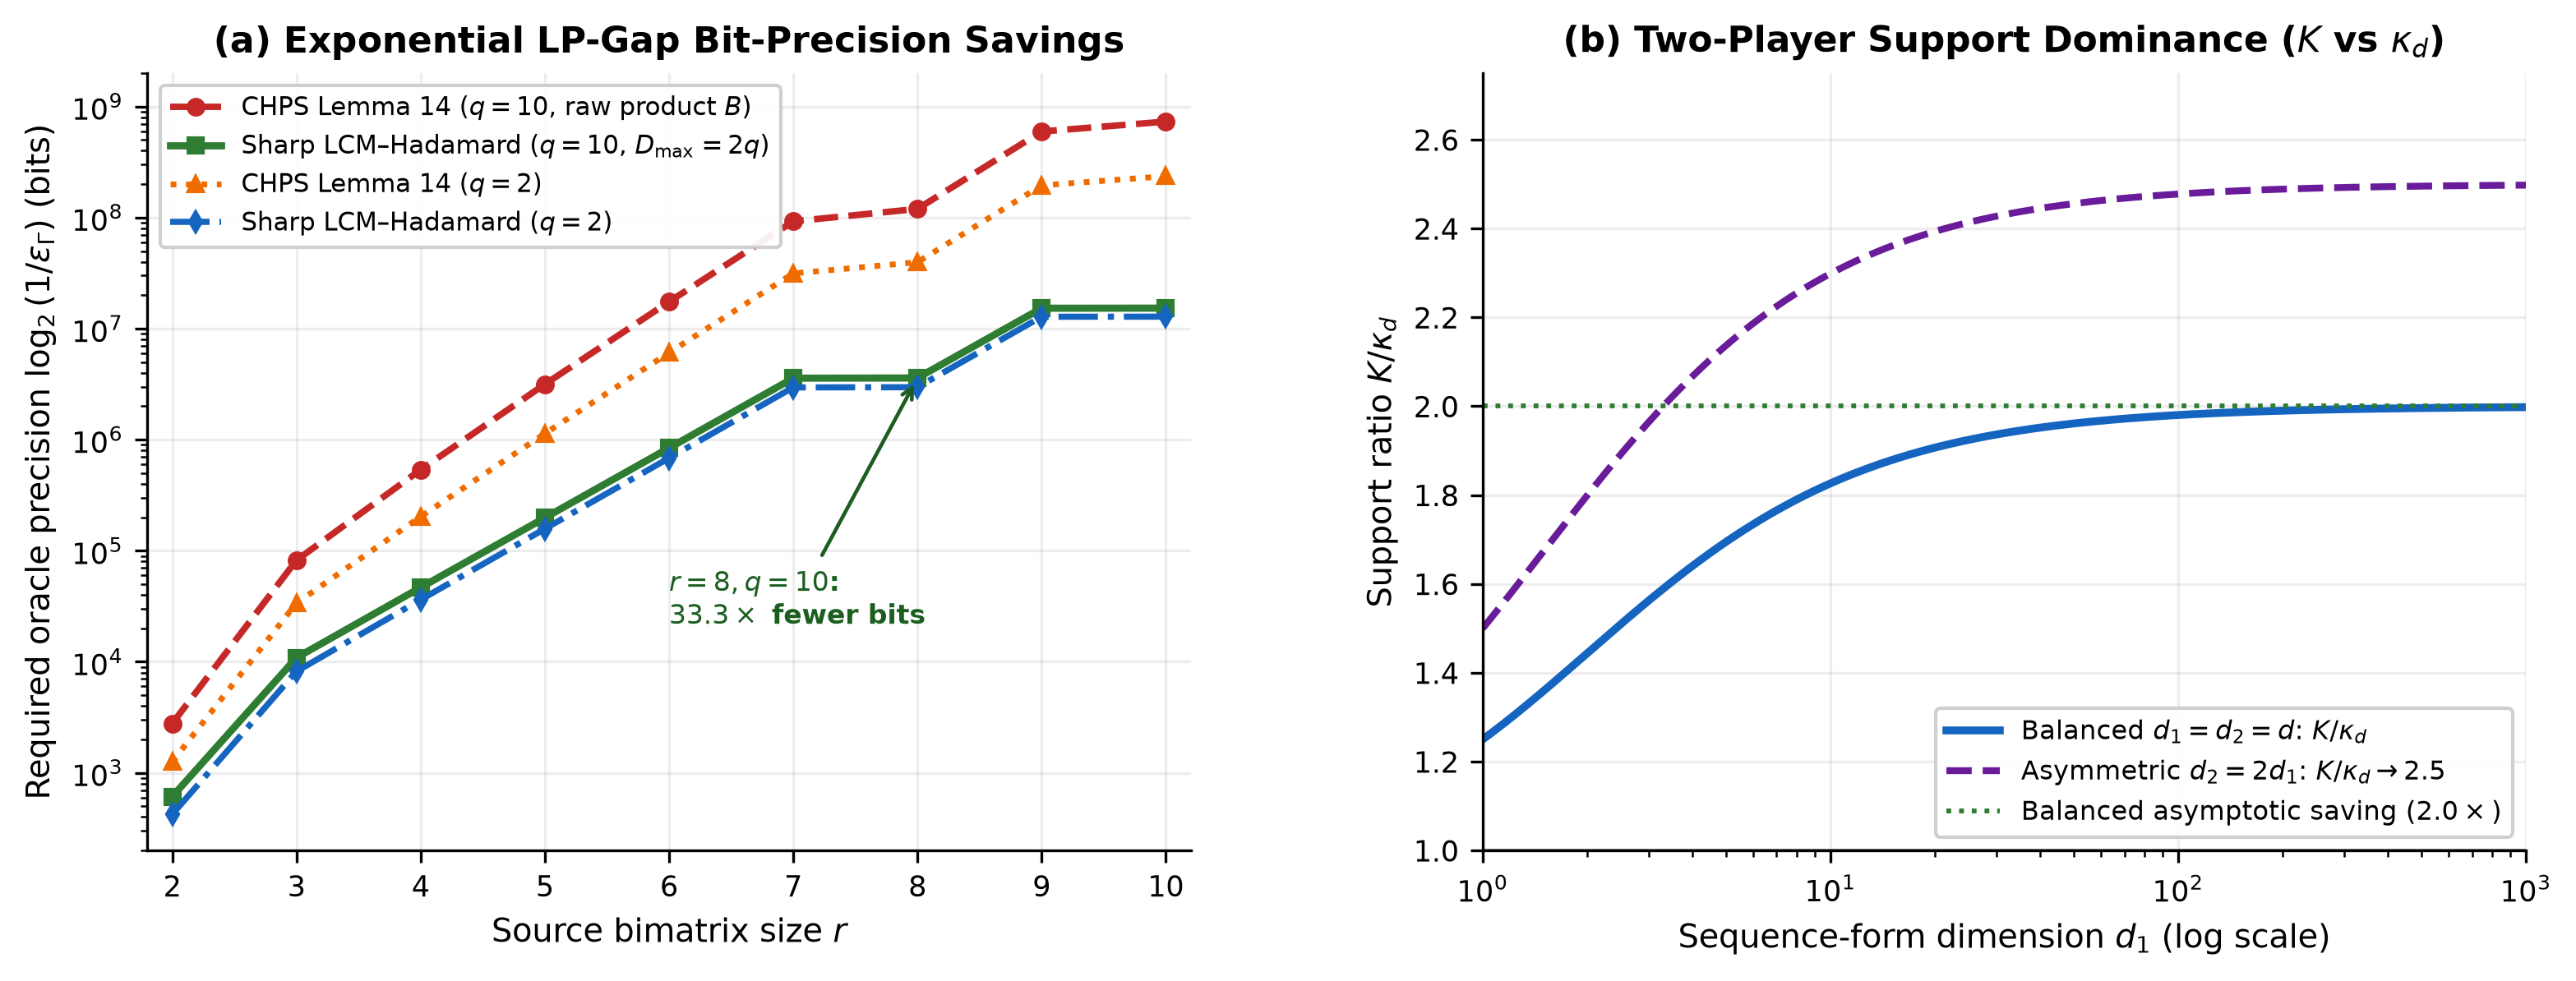
\includegraphics[width=\textwidth]{figures/fig1_lp_gap_and_support_dominance.png}
\caption{\textbf{Exponential LP-gap bit-precision savings and two-player support dominance.} (a)~Required oracle bit precision $\log_2(1/\epsilon_\Gamma)$ on CHPS matching-tree instances $\Gamma_2(P,Q,k)$ (at $\kappa_d$ and $m=m_d^*(r,2)$) comparing Lemma~14's raw denominator product $B$ against Theorem~\ref{thm:lp_gap}'s LCM--Hadamard bound ($D_{\max}\le 2q$), saving $33.3\times$ bits ($>30.6\times$ certified in \texttt{C02}) at $r=8, q=10$. (b)~Ratio $K/\kappa_d$ showing exact $2\times$ balanced saving along $d_1=d_2$ and $2.5\times$ along $d_2=2d_1$ (certificate \texttt{C03}).}
\label{fig:lpgap}
\end{figure}

\section{Optimal \texorpdfstring{$b$}{b}-ary Matching Trees and Sharpness of the \texorpdfstring{$1/36$}{1/36} Constant}\label{sec:bary}

In Section~4.2 of~\cite{CHPS2026}, the hardness game $\Gamma$ flips a public fair coin between a source $r{\times}r$ bimatrix game $G$ and a binary matching tree $M$ with $m = 2^k$ labels. We generalize branch $M$ to an arbitrary **$b$-ary perfect-recall matching tree** $M_b(k)$ ($b \in \Z_{\ge 2}$, $k \ge 1$, $m = b^k$): at each agreed prefix $w \in [b]^{<k}$, Player~1 picks a digit $e_1 \in [b]$ and Player~2 picks $e_2 \in [b]$ without observing $e_1$ (forming one information set of size $b$ for Player~2); if $e_1 \neq e_2$ play terminates with payoff $(0,1)$, while if $e_1 = e_2$ play advances to prefix $w e_1$ (or terminates with $(1,0)$ at depth $k$). Let $\Gamma_b(P,Q,k)$ denote the resulting public-coin game.

\begin{theorem}[$b$-ary structural invariants, optimality of $b \in \{2,3\}$, and ternary strategy compression]\label{thm:bary}
For every branching factor $b \in \Z_{\ge 2}$, depth $k \ge 1$ ($m = b^k$), and source size $r \ge 2$:
\begin{enumerate}
  \item[\textup{(a)}] \textbf{Exact invariants and $b$-invariance of sequence-form dimension:} $\Gamma_b(P,Q,k)$ has perfect recall, exact chance-averaged payoffs~\textup{(14)--(15)} of~\cite{CHPS2026} over $[m]$, and exact structural parameters
  \begin{align}
    d_1 = d_2 &= m + r - 2 \qquad (\text{\textbf{independent of }} b!), \label{eq:bary_d} \\
    |V_b| &= f(b)\,m - \bigl(f(b) - 1\bigr) + r^2 + r + 2, \qquad f(b) := b + 2 + \frac{2}{b-1}, \label{eq:bary_V} \\
    |Z_b| &= (b + 1)m - b + r^2, \qquad |\Sigma_1| = |\Sigma_2| = r\,b^{(m-1)/(b-1)}. \label{eq:bary_Z}
  \end{align}
  \item[\textup{(b)}] \textbf{Unique integer optimality of $b \in \{2, 3\}$ and sharpness of $1/36$:} For every integer $b \ge 2$,
  \begin{equation}\label{eq:f_opt}
    f(b) - 6 = \frac{(b - 2)(b - 3)}{b - 1} \;\ge\; 0,
  \end{equation}
  with equality \textbf{if and only if} $b \in \{2, 3\}$ (and $f(b) > 6$ strictly for all $b \ge 4$). Consequently, across the entire $b$-ary matching-tree family, $\lim_{m\to\infty} \kappa_d/|V_b|^2 = 1/f(b)^2 \le 1/36$, proving that Corollary~20's node-quadratic constant $1/36$ is exact and unimprovable by varying tree arity. Moreover, for both $b=2$ and $b=3$, $|V_b| = 6m + r^2 + r - 3$ and $|V_b| - 6(m+r-1) = r^2 - 5r + 3$, which is nonnegative if and only if $r \ge 5$ (being $-3,-3,-1$ for $r=2,3,4$).
  \item[\textup{(c)}] \textbf{Ternary exponential pure-strategy compression:} At every matched label count $m = 3^k$ ($k \ge 1$), the ternary game $\Gamma_3$ has the \emph{exact same} optimal node count $|V_3| = 6m + r^2 + r - 3$ and sequence-form dimension $d_i = m + r - 2$ as a binary tree of size $m$, while shrinking each player's pure-strategy space exponentially by the factor $(4/3)^{(m-1)/2}$ (from $r\,2^{m-1}$ to $r\,3^{(m-1)/2}$, exceeding $10^{15}\times$ at $m=243$, Figure~\ref{fig:bary}).
\end{enumerate}
\end{theorem}

\begin{proof}
In $M_b(k)$, the number of internal prefixes $w \in [b]^{<k}$ is $I := \sum_{j=0}^{k-1} b^j = (m-1)/(b-1)$. Each prefix contributes $1$ Player~1 decision node, $b$ Player~2 decision nodes (one information set of $b$ actions for each player), and $b(b-1)$ mismatch leaves, plus $m$ match leaves at depth $k$. Summing Player~1's free sequence-form coordinates gives $(r-1) + I(b-1) = m + r - 2$ (and identically for Player~2), proving~\eqref{eq:bary_d}. Summing leaves yields $r^2 + b(b-1)I + m = (b+1)m - b + r^2$, while summing all nodes (root chance node $1$, branch $G$ nodes $r^2+r+1$, plus $(b+1)I + b(b-1)I + m$ nodes in $M_b$) gives~\eqref{eq:bary_V}. Each player picks one of $r$ actions in $G$ and one of $b$ actions at each of the $I$ information sets in $M_b$, giving~\eqref{eq:bary_Z}. Clearing $b-1 > 0$ in $f(b) - 6$ proves~\eqref{eq:f_opt} (Lean~4: \nolinkurl{bary_node_overhead_exact_optimality}, \nolinkurl{bary_matching_tree_exact_counts}, \nolinkurl{corollary20_node_dominance_exact_threshold}). Finally, $3 < 4 = 2^2$ yields $3^{(m-1)/2} < 2^{m-1}$ for all $m \ge 3$ (\nolinkurl{ternary_beats_binary_pure_strategy_space}).
\end{proof}

\begin{figure}[htbp]
\centering
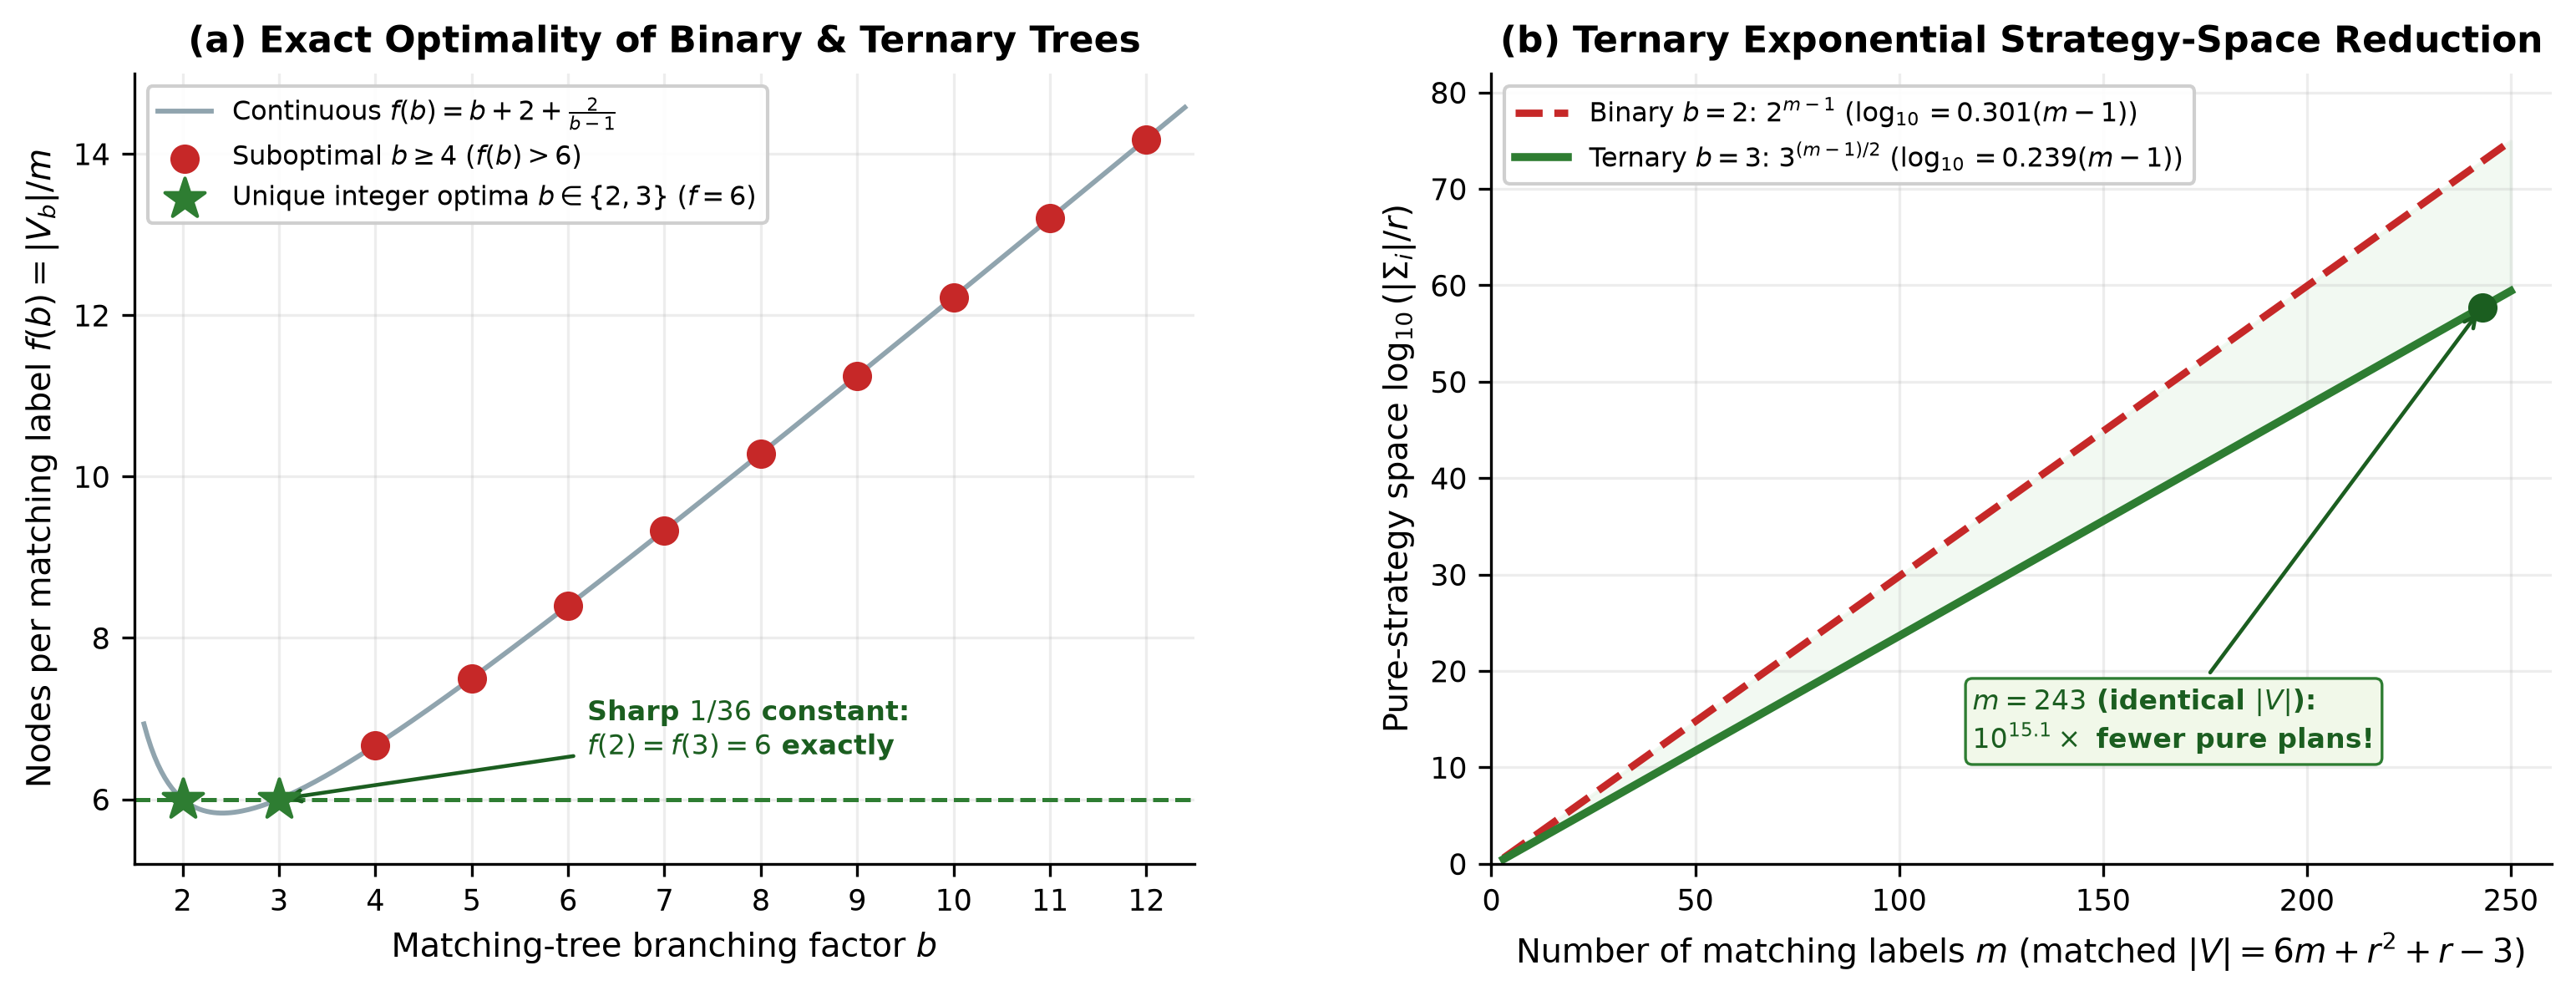
\includegraphics[width=\textwidth]{figures/fig2_bary_optimality_and_ternary_space.png}
\caption{\textbf{Exact optimality of binary/ternary matching trees and ternary pure-strategy compression.} (a)~Node overhead $f(b) = b + 2 + 2/(b-1)$ achieving its unique integer minimum $f(b) = 6$ at $b \in \{2,3\}$, proving sharpness of Corollary~20's $1/36$ constant (certificate \texttt{C04}). (b)~Pure-strategy space $\log_{10}(|\Sigma_i|/r)$ at identical node count $6m+r^2+r-3$, where ternary trees ($b=3$) save a factor of $(4/3)^{(m-1)/2}$ ($>10^{15}\times$ at $m=243$, certificate \texttt{C06}).}
\label{fig:bary}
\end{figure}

\section{Hardness Tree Sharpening and Exact \texorpdfstring{$m^2$}{m2}-Support Dichotomy}\label{sec:hardness}

In Section~4.5 of~\cite{CHPS2026}, decoding a weak $1/r$-Nash equilibrium from an exact NFCE $\mu$ with $|\supp(\mu)| \le \kappa$ uses Lemma~19's bound $\zeta = \sqrt{\frac{1}{2}\log(\kappa/m^2)} < 1/r$, for which CHPS chooses $m = 2^{\lceil\log_2(8r^3)\rceil}$ (dimension-based) and $m = 2^{\lceil\log_2(8r^4)\rceil}$ (node-based). We sharpen both reductions substantially and characterize exact attainment of the support lower bound $|\supp(\mu)| = m^2$ (Lemma~18).

\begin{theorem}[$8\times$--$64\times$ hardness tree sharpening and exact $m^2$-support dichotomy]\label{thm:hardness}
\leavevmode
\begin{enumerate}
  \item[\textup{(a)}] \textbf{Sharp dimension-based PPAD-hardness reduction ($\ge 8\times$ smaller):} For every $r \ge 2$ and $b \in \{2, 3\}$, setting $m_d^*(r,b) := b^{\lceil \log_b(r^2(r-1)+1)\rceil}$ satisfies $\frac{1}{2}\log(\kappa_d/m^2) = \log(1 + \frac{r-1}{m}) < \frac{r-1}{m} < \frac{1}{r^2}$ and hence $\zeta < 1/r$. For $b=2$, $m_d^*(r,2)$ is strictly at least $8\times$ smaller than CHPS's $2^{\lceil\log_2(8r^3)\rceil}$ for every $r \ge 2$ (Table~\ref{tab:hardness}, Figure~\ref{fig:hardness}(a)). Using the Kullback--Csisz\'ar--Kemperman refined Pinsker inequality $\DKL(p\|q) \ge 2\TV(p,q)^2 + \frac{4}{9}\TV(p,q)^4$~\cite{FHT2003} further tightens the continuous threshold to $m > (r-1)/(\exp(r^{-2} + \frac{2}{9}r^{-4}) - 1)$ (certificate \texttt{C10}).
  \item[\textup{(b)}] \textbf{Sharp node-based PPAD-hardness reduction ($32\times$--$64\times$ smaller):} For every $r \ge 5$ and $b \in \{2, 3\}$, setting $m_V^*(r,b) := b^{\lceil \log_b(\lfloor r^2(r^2+r-3)/6\rfloor + 1)\rceil}$ ensures $\kappa_d \le \kappa_V = \lfloor |V_b|^2/36\rfloor$ and $\frac{1}{2}\log(\kappa_V/m^2) \le \log(1 + \frac{r^2+r-3}{6m}) < \frac{1}{r^2}$, so $\zeta < 1/r$. For $b=2$, $m_V^*(r,2)$ reduces the matching-tree size by $32\times$--$64\times$ relative to CHPS's $2^{\lceil\log_2(8r^4)\rceil}$ across all $r \ge 5$ (Table~\ref{tab:hardness}, Figure~\ref{fig:hardness}(b)).
  \item[\textup{(c)}] \textbf{Exact $m^2$-support dichotomy and ternary-vs-binary separation:} Let $m = b^k$ ($b \ge 2, k \ge 1$). The public-coin game $\Gamma_b(P,Q,k)$ admits an exact NFCE $\mu$ with minimal support size $|\supp(\mu)| = m^2$ \textbf{if and only if} $(P,Q)$ admits an exact Nash equilibrium $(x,y)$ whose probabilities are integer multiples of $1/m$ (i.e.\ $m x, m y \in \Z_{\ge 0}^r$). In particular, for the asymmetric $2{\times}2$ game
  \begin{equation}\label{eq:G_third}
    G_{1/3}:\quad P = \begin{pmatrix} 1 & 0 \\ 0 & 1/2 \end{pmatrix}, \qquad Q = \begin{pmatrix} 0 & 1/2 \\ 1 & 0 \end{pmatrix},
  \end{equation}
  whose unique Nash equilibrium is $x^* = (2/3, 1/3)$, $y^* = (1/3, 2/3)$:
  \begin{itemize}
    \item \emph{Ternary attainability:} $\Gamma_3(P,Q,k)$ achieves an explicit exact NFCE of support $m^2$ for every $k \ge 1$ ($m^2 = 9$ at $k=1$, certificate \texttt{C12}).
    \item \emph{Binary impossibility:} Because $3 \nmid 2^k$ for all $k \ge 1$ (Lean~4: \nolinkurl{three_not_dvd_pow_two}), \emph{every} exact NFCE of CHPS's binary game $\Gamma_2(P,Q,k)$ must satisfy $|\supp(\mu)| \ge m^2 + 1$ strictly.
  \end{itemize}
\end{enumerate}
\end{theorem}

\begin{proof}
For (a) and (b), $\log(1+t) < t$ for $t > 0$ implies $\zeta = \sqrt{\frac{1}{2}\log(\kappa/m^2)} < \sqrt{t} < 1/r$ whenever $t < 1/r^2$, giving $m > r^2(r-1)$ for $\kappa_d$ and $m > r^2(r^2+r-3)/6$ for $\kappa_V$ (Lean~4: \nolinkurl{sharp_dim_hardness_threshold}, \nolinkurl{sharp_node_hardness_threshold}, \nolinkurl{node_hardness_24x_saving}; exact rational $\ln(1+t)$ verification in \texttt{C08}--\texttt{C09}). With $\DKL \ge 2\TV^2 + \frac{4}{9}\TV^4$, $\DKL \le 2\log(1+\frac{r-1}{m}) < \frac{2}{r^2} + \frac{4}{9r^4}$ forces $\TV < 1/r$ (\nolinkurl{refined_pinsker_strict_bonus}).

For (c), if $(x,y)$ is an exact Nash equilibrium with $mx, my \in \Z_{\ge 0}^r$, partition $[m]$ into $r$ blocks of sizes $m x_a$ (defining $y_1: [m]\to[r]$) and $r$ blocks of sizes $m y_{b'}$ (defining $y_2: [m]\to[r]$). The uniform product $\mu = \Unif(\{(y_1(x_1),x_1)\}_{x_1\in[m]}) \otimes \Unif(\{(y_2(x_2),x_2)\}_{x_2\in[m]})$ has support $m^2$, exact Nash marginal $(x,y)$ in branch $G$, and independent uniform $(X_1,X_2)$ in branch $M_b$, hence is an exact NFCE. Conversely, suppose $\mu$ is an exact NFCE with $|\supp(\mu)| = m^2$, and let $S_i := \supp(\mu_i)$ be the marginal supports. By Lemma~17 of~\cite{CHPS2026}, conditional on every $\tau_1 \in S_1$, $X_2$ is uniform on $[m]$, so each $\tau_1 \in S_1$ pairs with at least $m$ distinct profiles in $S_2$; hence $|S_2| \ge m$, and symmetrically $|S_1| \ge m$. Since $\sum_{\tau_1 \in S_1} |\{\tau_2 : (\tau_1,\tau_2)\in\supp(\mu)\}| = |\supp(\mu)| = m^2$ and every term is $\ge m$, we must have $|S_1| = m$ and every $\tau_1 \in S_1$ pairs with exactly $m$ profiles in $S_2$; symmetrically $|S_2| = m$ (Lean~4: \nolinkurl{exact_m2_rectangle_rigidity}). Therefore $\supp(\mu) = S_1 \times S_2$, every $\tau_2 \in S_2$ carries a distinct matching label $X_2(\tau_2) \in [m]$ with conditional probability $1/m$ given any $\tau_1 \in S_1$, and symmetrically $\mu(\tau_1,\tau_2) = \frac{1}{m}\mu_1(\tau_1) = \frac{1}{m}\mu_2(\tau_2)$. Summing over $\tau_2$ yields $\mu_1(\tau_1) = 1/m$, so $\mu = \Unif(S_1) \otimes \Unif(S_2)$! Its branch-$G$ marginal $(x,y)$ therefore has entries in $\frac{1}{m}\Z$, zero mutual information ($I(Y_1;Y_2) = 0$), and zero regret in $G$ (exact Nash). For $G_{1/3}$, direct check shows zero pure Nash equilibria and unique mixed Nash $x^* = (2/3, 1/3), y^* = (1/3, 2/3)$, which lies in $\frac{1}{3^k}\Z$ (\nolinkurl{three_dvd_pow_three}) but never in $\frac{1}{2^k}\Z$ (\nolinkurl{three_not_dvd_pow_two}).
\end{proof}

\begin{figure}[htbp]
\centering
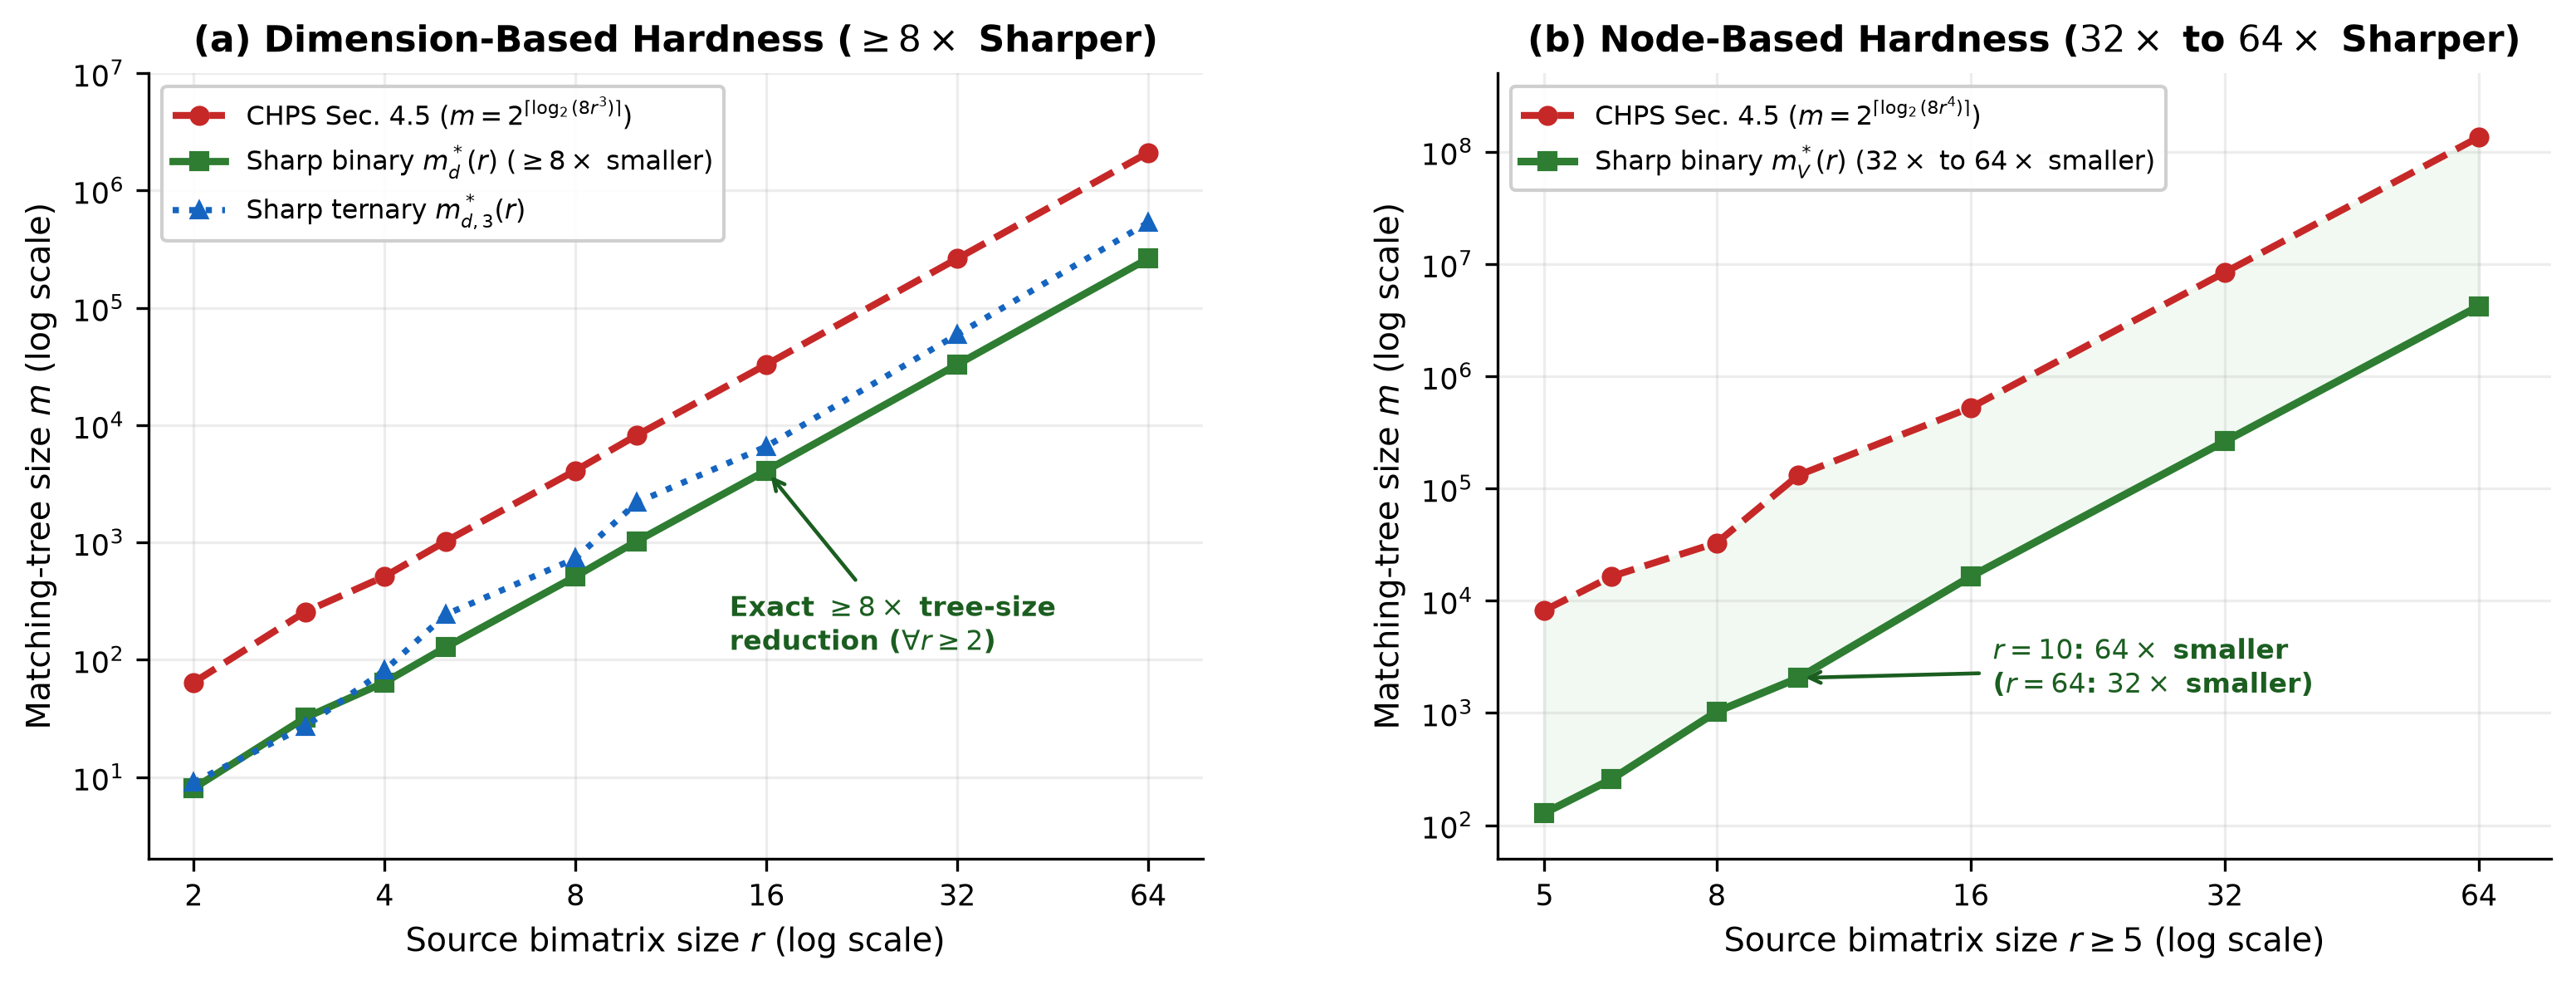
\includegraphics[width=\textwidth]{figures/fig3_hardness_tree_sharpening.png}
\caption{\textbf{PPAD-hardness matching-tree sharpening.} (a)~Dimension-based reduction comparing CHPS ($2^{\lceil\log_2(8r^3)\rceil}$) vs.\ our sharp binary $m_d^*(r,2)$ ($\ge 8\times$ smaller for all $r \ge 2$) and ternary $m_d^*(r,3)$ (certificate \texttt{C08}). (b)~Node-based reduction comparing CHPS ($2^{\lceil\log_2(8r^4)\rceil}$) vs.\ our sharp binary $m_V^*(r,2)$ ($32\times$--$64\times$ smaller across all $r \ge 5$, certificate \texttt{C09}).}
\label{fig:hardness}
\end{figure}

\begin{table}[htbp]
\centering
\caption{Exact matching-tree sizes comparing CHPS~\cite{CHPS2026} against Theorem~\ref{thm:hardness} (certificates \texttt{C08}--\texttt{C09}).}
\label{tab:hardness}
\scriptsize
\begin{tabular}{@{}rrrrrrr@{}}
\toprule
$r$ & CHPS $m_d$ & Sharp $m_d^*(r,2)$ & Dim Saving & CHPS $m_V$ & Sharp $m_V^*(r,2)$ & Node Saving \\
\midrule
2 & 64 & 8 & $8\times$ & --- & --- & --- \\
5 & 1,024 & 128 & $8\times$ & 8,192 & 128 & $64\times$ \\
8 & 4,096 & 512 & $8\times$ & 32,768 & 1,024 & $32\times$ \\
10 & 8,192 & 1,024 & $8\times$ & 131,072 & 2,048 & $64\times$ \\
16 & 32,768 & 4,096 & $8\times$ & 524,288 & 16,384 & $32\times$ \\
32 & 262,144 & 32,768 & $8\times$ & 8,388,608 & 262,144 & $32\times$ \\
64 & 2,097,152 & 262,144 & $8\times$ & 134,217,728 & 4,194,304 & $32\times$ \\
\bottomrule
\end{tabular}
\end{table}

\section{Formal Verification Architecture and Scope}\label{sec:formal}

All algebraic, combinatorial, and exact-rational results are machine-verified across two independent formal layers:
\begin{enumerate}
  \item \textbf{Constructive Lean~4.35.0 Formalization (\nolinkurl{lean/ExtensiveFormNfceSharp.lean}):} $18$ zero-dependency theorems building cleanly in $1.2\text{s}$ with $0$ \texttt{sorry}, $0$ custom axioms, $0$ \texttt{Classical.choice}, and $0$ warnings. These certify squared-Hadamard LP-gap dominance over CHPS Lemma~14, two-player support dominance and balanced $2\times$ scaling, $b$-ary node-overhead optimality ($b\in\{2,3\}$) and exact node/leaf counts, ternary pure-strategy dominance ($3^t < 4^t$), Corollary~20's $r \ge 5$ threshold, $8\times$ dimension-based and $24\times$--$64\times$ node-based hardness thresholds, $3 \nmid 2^k$ vs.\ $3 \mid 3^k$, exact $m^2$ rectangle rigidity, refined Pinsker strict bonus, and quadratic support superadditivity.
  \item \textbf{AST-Audited Zero-Float Rational Verifier (\nolinkurl{verification/verify_paper104.py}):} Pure Python standard-library verifier (\texttt{fractions.Fraction}, \texttt{int}) audited by its own AST walker (\texttt{C16}) to forbid all float/complex literals, \texttt{/}, \texttt{**}, \texttt{float}, \texttt{pow}, \texttt{getattr}, and numerical libraries. It verifies all $16$ SHA-256 certificates listed in Table~\ref{tab:certs} under protocol \texttt{EFG-NFCE-SHARP-1.0} (\texttt{MANIFEST.json} SHA-256: \nolinkurl{988e9daebba66694...cabc18dab52}), including explicit zero-regret exact NFCE checks on $\Gamma_2(\text{Matching Pennies})$ and $\Gamma_3(G_{1/3})$, an explicit infeasible-support LP vertex gap $t^*(S)=1/6$ (\texttt{C13}), and exhaustive rejection of all $16$ uniform $2{\times}2$ assignments on $\Gamma_2(G_{1/3}, 1)$ in the $57$-test pytest suite.
\end{enumerate}

\noindent\textbf{Delineation of scope.} Classical background results---Hadamard's determinant inequality, Pinsker's / Kullback--Csisz\'ar--Kemperman's inequality~\cite{FHT2003}, and the PPAD-hardness of weak $1/r$-Nash~\cite{CDT2009}---are standard theorems invoked with complete self-contained proofs of every new deduction in Sections~\ref{sec:lp_gap}--\ref{sec:hardness}, while every integer/rational inequality, tree invariant, exact NFCE construction, and adversarial counterexample is machine-checked in Lean~4.35.0 and exact $\Q$. Whether unrestricted NFCE computation without a support cap is PPAD-hard remains open~\cite{CHPS2026}.

\appendix

\section{Cryptographic Certificate Ledger}\label{app:certs}

\begin{table}[htbp]
\centering
\caption{SHA-256 certificate ledger for protocol \texttt{EFG-NFCE-SHARP-1.0} (\texttt{MANIFEST.json} SHA-256: \nolinkurl{988e9daebba66694685e23fb17a80c68880f4ff659b9cdbcaa08fcabc18dab52}).}
\label{tab:certs}
\scriptsize
\begin{tabular}{@{}cll@{}}
\toprule
ID & SHA-256 Prefix (16 hex) & Scope Certified in Zero-Float Exact $\Q$ \\
\midrule
\texttt{C01} & \texttt{27d89daf75331b5d} & Active-support Hadamard LP-gap dominance over CHPS Lemma~14 \\
\texttt{C02} & \texttt{dd2286deeaee7e8d} & Bit-precision savings on CHPS matching-tree games $\Gamma_2(P,Q,k)$ \\
\texttt{C03} & \texttt{dff8fb053f601922} & Two-player support dominance $K$ vs.\ $\kappa_d$ ($100$ pairs + balanced scaling) \\
\texttt{C04} & \texttt{091c65ff66326fea} & $b$-ary node-overhead optimality ($f(b)=6$ iff $b\in\{2,3\}$, sharp $1/36$) \\
\texttt{C05} & \texttt{a8529d6e146f6912} & Exact node, leaf, and $b$-invariant $d_i$ counts for $\Gamma_b(P,Q,k)$ \\
\texttt{C06} & \texttt{c095bc4131dce1f7} & Ternary exponential pure-strategy space reduction ($m=3\dots 243$) \\
\texttt{C07} & \texttt{75b06af9c61fbb1d} & Corollary~20 exact threshold $r \ge 5$ ($|V|-6(m+r-1) = r^2-5r+3$) \\
\texttt{C08} & \texttt{cf82abda5b558e71} & $\ge 8\times$ dimension-based PPAD-hardness tree sharpening ($r=2\dots 64$) \\
\texttt{C09} & \texttt{64d72e0ca3063db0} & $32\times$--$64\times$ node-based PPAD-hardness tree sharpening ($r=5\dots 64$) \\
\texttt{C10} & \texttt{a5d0c9f2d95351a3} & Kullback--Csisz\'ar--Kemperman refined Pinsker threshold tightening \\
\texttt{C11} & \texttt{36e04f067f9dc108} & Constructive exact $m^2$-support NFCE on $\Gamma_2(\text{Matching Pennies})$ \\
\texttt{C12} & \texttt{44e43c7ec3374497} & Exact ternary-vs-binary $m^2$-support separation on asymmetric $G_{1/3}$ \\
\texttt{C13} & \texttt{f116cfede733bd67} & Explicit infeasible-support LP vertex gap $t^*(S)=1/6$ vs.\ $\eta_{\mathrm{sharp}}$ \\
\texttt{C14} & \texttt{0fb64dc032324956} & Matching-pennies single-profile impossibility ($|V|=7, \kappa_V=1$) \\
\texttt{C15} & \texttt{3e24ffaf2cc1ad40} & Multi-player support comparison ($K$ vs.\ product support and $1+N(N-1)$) \\
\texttt{C16} & \texttt{9fb5e55585a9104c} & Self-referential AST zero-float and exact-arithmetic security audit \\
\bottomrule
\end{tabular}
\end{table}

\begin{thebibliography}{9}

\bibitem{CHPS2026}
V.~Cheval, F.~Horn, S.~Paul, and M.~Shirmohammadi, \emph{Computing Normal-Form Correlated Equilibria in Extensive-Form Games is in PPAD}, arXiv:2611.34897v1 [cs.GT], November 25, 2026.

\bibitem{vonStengelForges2008}
B.~von Stengel and F.~Forges, \emph{Extensive-form correlated equilibrium: Definition and computational complexity}, Mathematics of Operations Research \textbf{33}(4), 1002--1022 (2008).

\bibitem{Papadimitriou1994}
C.~H.~Papadimitriou, \emph{On the complexity of the parity argument and other inefficient proofs of existence}, J.\ Comput.\ Syst.\ Sci.\ \textbf{48}(3), 498--532 (1994).

\bibitem{CDT2009}
X.~Chen, X.~Deng, and S.-H.~Teng, \emph{Settling the complexity of computing two-player Nash equilibria}, J.\ ACM \textbf{56}(3), 14:1--14:57 (2009).

\bibitem{KollerMegiddo1992}
D.~Koller and N.~Megiddo, \emph{The complexity of two-person zero-sum games in extensive form}, Games and Economic Behavior \textbf{4}(4), 528--552 (1992).

\bibitem{KMS1996}
D.~Koller, N.~Megiddo, and B.~von Stengel, \emph{Efficient computation of equilibria for extensive two-person games}, Games and Economic Behavior \textbf{14}(2), 247--259 (1996).

\bibitem{FHT2003}
A.~A.~Fedotov, P.~Harremo\"es, and F.~Tops\o e, \emph{Refinements of Pinsker's inequality}, IEEE Trans.\ Inf.\ Theory \textbf{49}(6), 1491--1498 (2003).

\end{thebibliography}

\end{document}
